To create a TikZ LaTeX diagram that represents topologically equivalent but geometrically distinct partitions of an annulus \(X\), we can use the following code:

```latex
\documentclass{standalone}
\usepackage{tikz}

\begin{document}

% Define colors for clarity
\definecolor{red}{RGB}{255,0,0}
\definecolor{green}{RGB}{0,255,0}
\definecolor{blue}{RGB}{0,0,255}
\definecolor{yellow}{RGB}{255,255,0}

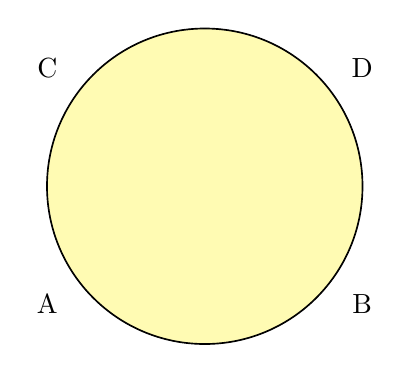
\begin{tikzpicture}[scale=2]

% Draw the outer circle of the annulus
\draw[thick] (0,0) circle (1);

% Draw the inner circle of the annulus
\draw[thick] (0,0) circle (0.5);

% Define the points for partitioning
\node at (-0.866, -0.5) (A) {};
\node at (0.866, -0.5) (B) {};
\node at (-0.866, 0.5) (C) {};
\node at (0.866, 0.5) (D) {};

% Draw the segments for partitioning
\draw[dashed, red] (A) -- (B);
\draw[dashed, green] (B) -- (D);
\draw[dashed, blue] (D) -- (C);
\draw[dashed, yellow] (C) -- (A);

% Label the segments
\node at (-1, -0.75) {A};
\node at (1, -0.75) {B};
\node at (-1, 0.75) {C};
\node at (1, 0.75) {D};

% Draw the circles for the partitions
\filldraw[fill=red!30] (0,0) circle (0.4);
\filldraw[fill=green!30] (0,0) circle (0.6);
\filldraw[fill=blue!30] (0,0) circle (0.8);
\filldraw[fill=yellow!30] (0,0) circle (1);

\end{tikzpicture}

\end{document}
``